\newpage
\section{Daten-Pipeline}
\label{chapter:daten_pipeline}
\subsection{Bilder aufnehmen}
\label{chapter:bilder_aufnehmen}
Die Aufnahme der Bilder geschah unverändert mit der Apparatur und dem C++ Code von Tabea Méndez welche aus Ihrer Masterarbeit \cite{TabeasFingertracking} entstanden. 
Das Ergebnis bestand jeweils aus acht Bildern von einer Situation. 
Eine Situation bestand aus vier Kameras.
Dabei machte jede Kamera jeweils ein schwarzweiss-Bild mit UV-Beleuchtung und ein schwarzweiss-Bild mit normaler weisser Beleuchtung.
Als die Daten gelablet wurden, wurden noch keine Zeitinformation verwendet.
Das heisst die Finger wurden noch nicht von Bild zu Bild getrackt.
So wurden helle Punkte im Hintergrund oft als Finger erkannt.
Um dies zu umgehen wurde der Aufbau im Hintergrund mit schwarzem Papier abgedeckt.

Pro Durchgang konnten maximal 6000 Situationen aufgenommen werden, bevor der Arbeitsspeicher des dafür verwendeten Computers an seine Grenzen kam. 
Eine Verbesserung könnte hier erreicht werden, wenn man das Programm in zwei verschiedene Threads aufteilen würde.
Dabei wäre ein Thread für das Aufnehmen der Daten und der andere für das Abspeichern zuständig.
So könnten \grqq{}zeitlich unbegrenzt\grqq{} Daten aufgenommen werden. 
Dies würde aber nur nötig, falls in Zukunft ein Roboter verwendet wird, um Daten aufzunehmen.

\subsection{Fingerdetektion}
\label{chapter:fingerdetektion}
\begin{figure}
	\centering
	\begin{minipage}[b]{0.48\textwidth}	
		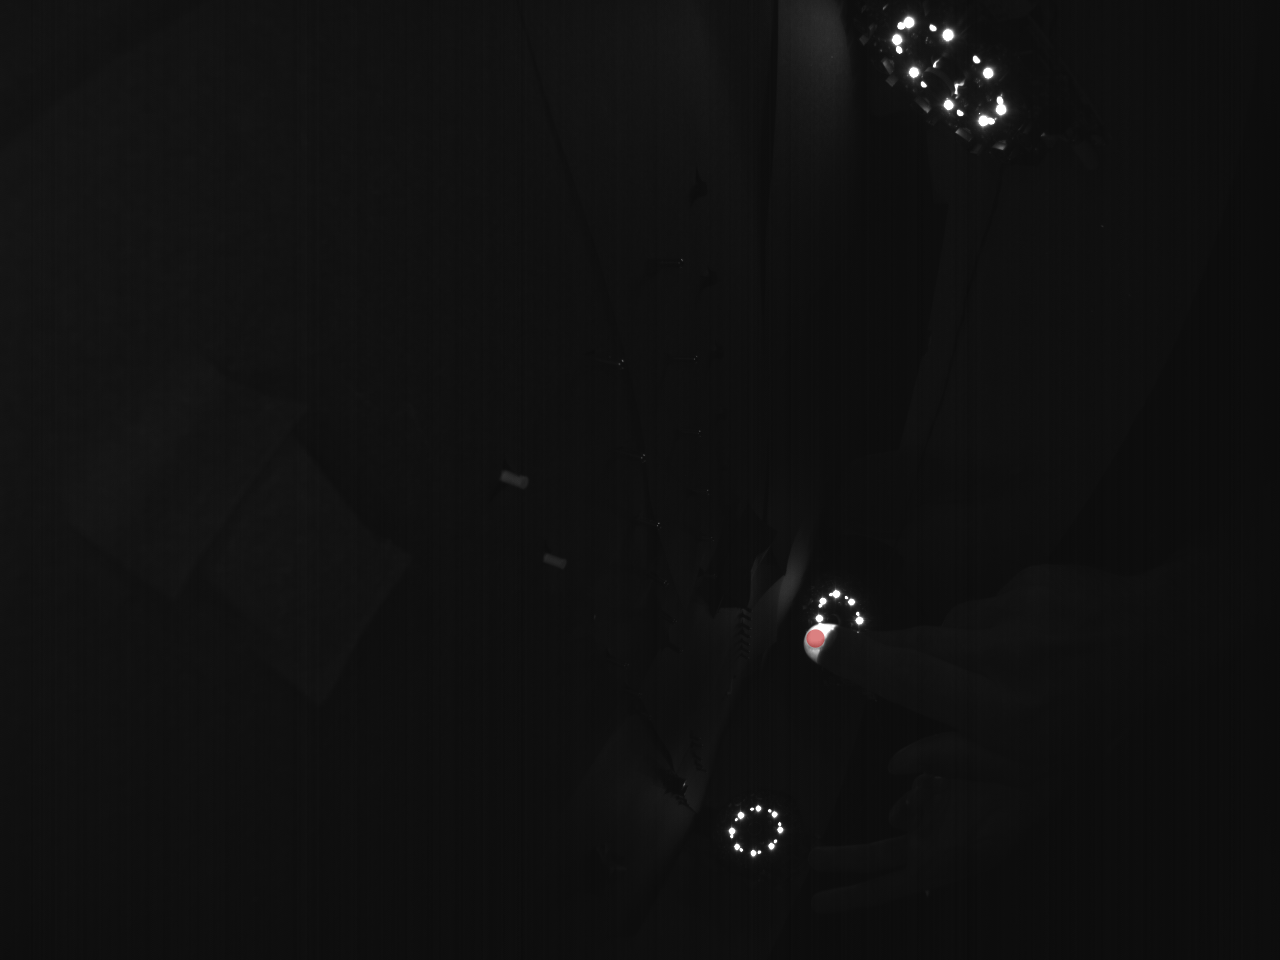
\includegraphics[trim = 270mm 90mm 90mm 170mm, clip, width=\textwidth]{Kapitel/30DatenPipeline/Bilder/schlechteBoundingboxen/pic775.png}
	\end{minipage}
	\hfill
	\begin{minipage}[b]{0.48\textwidth}		
		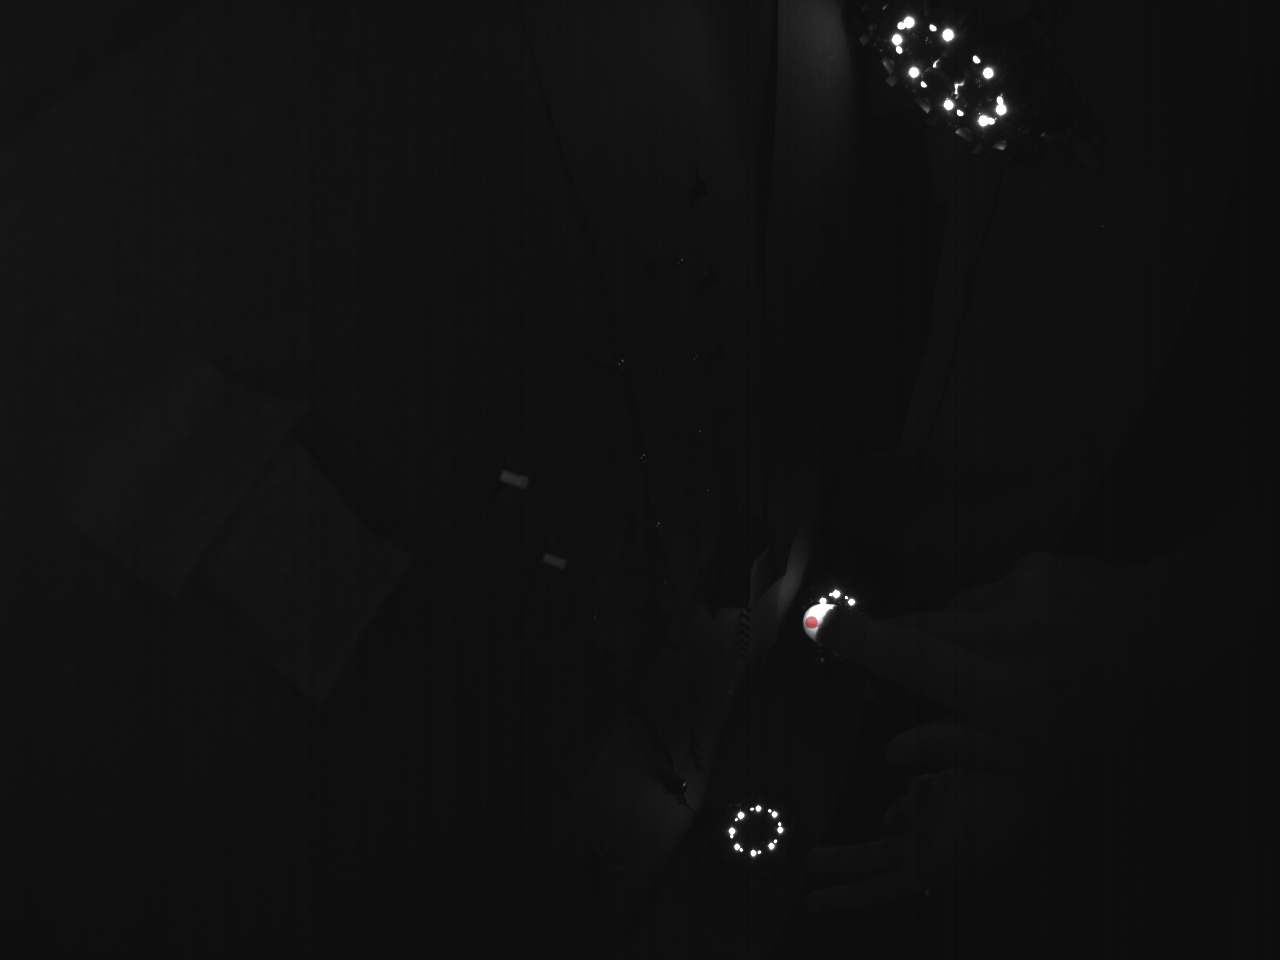
\includegraphics[trim = 270mm 90mm 90mm 170mm, clip,width=\textwidth]{Kapitel/30DatenPipeline/Bilder/schlechteBoundingboxen/pic777.png}
	\end{minipage}
	\caption{Resultate der Erosion}
	\label{img:Erosion}
\end{figure}
Zur Fingerdetektion wurde der Matlab-Fingerdetektor aus der Masterarbeit von Tabea Méndez \cite{TabeasFingertracking} verwendet. 
Um Zeit bei der Datenaufnahme einzusparen wurden Zeit- und Rauminformationen nicht miteinbezogen. 
Dies brachte einige neue Probleme mit sich.   
So wurden auch mit Restlicht beleuchtete Punkte im Hintergrund oder LED's, als Finger erkannt.
Dieses Problem konnte weitgehend behoben werden, indem in den Matlab-Fingerdetektor noch einige Filter eingebaut wurden.
Diese Filter hatten folgende Funktionen.
\begin{enumerate}
\item Überspringen von Bildern, welche eine gewisse Helligkeit überschreiten. 
Dies sortierte Bilder aus, welche eine grosse Hintergrundhelligkeit und dadurch auch viele fehlerhaft erkannten Fingerspitzen enthielten.  
\item Aussortieren von erkannten Punkten, welche zu gross waren, als dass Sie eine Fingerspitze sein könnten. 
Dieser Punkt ist teilweise redundant mit dem ersten Punkt, da grosse Punkte im Hintergrund oft nur bei einer extrem grossen Helligkeit auftreten können.  
\item Aussortieren von erkannten Punkten, welche zu klein waren, als dass Sie eine Fingerspitze sein konnten. 
Damit wurden die meisten LED-Punkte entfernt.
\item Von den übrigen Punkten wird dann nur noch der Grösste behalten.
Diesem wurde somit das Label \grqq{}rechter Zeigefingerspitz\grqq{} verliehen. 
\end{enumerate}
Mit diesen Filtern konnte ein hoher Prozentsatz der rechten Zeigefinger korrekt detektiert werden.
Auf den Finger selber bezogen, war die Genauigkeit leider jedoch relativ schlecht.
Es lag daran, dass die Detektionspunkte nicht immer genau in der Mitte des Fingers lagen. 
Weiter waren auch die Boundingboxen, welche sich aus dem Resultat der Erosion \cite{TabeasFingertracking} berechnen liessen nicht sehr genau. 
Wie man in der Abbildung \ref{img:Erosion} sehen kann, können sich diese innerhalb des Fingers auch bei sehr ähnlichen Bildern stark unterscheiden.

\subsection{CSV generieren}
Das Fingerspitzentracking wurde mit Matlab gemacht und die entsprechenden Labels als .mat-File abgespeichert.
Yolo hingegen wurde mit Tensorflow und entsprechend mit Python angegangen. 
Leider war es nicht möglich mit Python direkt .mat-Files zu öffnen. 
Aus diesem Grund wurde ein kleines Matlab-Skript erstellt, welches die Labels als CSV abspeicherte. 
In diesem Skript wurden ausserdem die Daten in Test und in Trainingsdaten aufgeteilt und je in einem seperaten CSV abgespeichert.
In diesem CSV gehört jedem Bild eine Zeile. 
Pro Zeile bzw. Bild werden folgende Punkte beschrieben:
\begin{enumerate}
\item Eindeutiger Bildname, mit welchem das Bild aus dem Directory geladen werden kann. 
\item X-Koordinaten im Range [0:1280]
\item Y-Koordinaten im Range [0:960]
\item Durchmesser des Resultats der Erosion
\item Wahrscheinlichkeit, dass ein rechter Zeigefinger in diesem Bild ist. 
(Entweder 1 oder 0, je nach dem, ob ein Finger erkannt wurde.)
\end{enumerate}


\subsection{Python-Objekt generieren}
Um die Daten einfach im Trainingsprozess aufrufen zu können, wurde eine kleine Python-Klasse geschrieben.
Die Daten mussten allerdings vor der Verwendung im Training durch eine Funktion dieser Klasse vorverarbeitet werden.
Die Gründe für die Vorverarbeitung sind: 
\begin{enumerate}
\item Die Bilder wurden bisher kameraweise bearbeitet.
Dies bedeutet, die Bilder hiessen bei verschiedenen Kameras genau gleich.
Mit der Vorverarbeitung wurden alle Bilder an einem gemeinsamen Ort gespeichert.
Ausserdem erhielt jedes Bild einen neuen Namen / eine neue Nummerierung, wodurch es möglich wurde sie eindeutig zuzuordnen. 
\item Um im Training einfach mit den Label-Daten umgehen zu können und um Rechenaufwand während dem Training zu sparen wurden in der Vorverarbeitung die Labels zu demjenigen Tensor zusammengefügt, welcher in Abbildung \ref{img:label_tensor} zu sehen ist.
\item Die Distanzen X und Y sowie die Höhe und Breite der Boundingbox mussten noch normalisiert werden, damit beim Training einfacher gerechnet werden kann.
\end{enumerate}
\subsubsection{Label-Tensor}
\label{chapter:label_tensor}
Die Labels pro Bild sind in einem Tensor angeordnet. 
(Siehe Abbildung \ref{img:label_tensor})
Diese Anordnung wurde stark am Output-Tensor wie er im Yolo-Paper \cite{yolo} erscheint angelehnt.
Dabei wird das Bild in ein 7x7 Raster aufgeteilt.
Für jedes Element dieses Gitternetzes werden folgende Punkte gespeichert:
\begin{labeling}{Label-Tensor}
\item[x] Die Distanz des Zentrums der Fingerspitze zum linken Rand der Gitterzelle.
Ist kein Finger in dieser Gitterzelle, ist diese Variable gleich Null.

Diese Variable ist folgendermassen normiert: 
Ist das Zentrum der Fingerspitze ganz links in der entsprechenden Gitterzelle, ist die Variable gleich null.
Ist das Zentrum der Fingerspitze ganz rechts in der entsprechenden Gitterzelle, ist die Variable gleich eins.
\item[y] Die Distanz des Zentrums der Fingerspitze zum oberen Rand der Gitterzelle.
Ist kein Finger in dieser Gitterzelle, ist diese Variable gleich Null. 

Diese Variable ist folgendermassen normiert:
Ist das Zentrum der Fingerspitze ganz oben in der entsprechenden Gitterzelle, ist die Variable gleich null.
Ist das Zentrum der Fingerspitze ganz unten in der entsprechenden Gitterzelle, ist die Variable gleich eins.
\item[h] Die Höhe der entsprechenden Bounding Box.
Ist kein Finger in dieser Gitterzelle, ist diese Höhe gleich null.

Diese Variable ist folgendermassen normiert:
Ist die Box insgesamt so hoch wie das Bild, ist diese Variable gleich eins. 
Ist die Box \grqq{}unendlich\grqq{} klein, so ist diese Variable gleich null.
\item[w] Die Breite der entsprechenden Bounding Box.
Ist kein Finger in dieser Gitterzelle, ist diese Höhe gleich null.

Diese Variable ist folgendermassen normiert:
Ist die Box insgesamt so breit wie das Bild, ist diese Variable gleich eins.
Ist die Box \grqq{}unendlich\grqq{} schmal, so ist diese Variable gleich null.
\item[p] Die Wahrscheinlichkeit, dass die Spitze eines rechten Zeigefingers in dieser Gitterzelle ist. 

Ist eine rechte Zeigefingerspitze in dieser Gitterzelle, so ist diese Variable gleich eins.
Ist keine rechte Zeigefingerspitze in dieser Gitterzelle, so ist diese Variable gleich null.

In diesem vereinfachten Fall gibt es nur eine p-Schicht.
(Weil nur der rechte Zeigefingerspitz gelabelt wurde.)
Wären aber auf dem Bild alle Finger einzeln gelabelt, müsste der Labeltensor für jeden zusätzlich labelbaren Finger eine weitere Schicht p haben. 
Würden also alle 10 Finger eines Menschen gelabelt, müsste der Labeltensor entsprechend 10 verschiedene p-Schichten haben.
(Die Anzahl x, y, h \& w - Schichten bleibt gleich) 
\end{labeling}

%Label-Tensor
\begin{figure}	
	\centering
	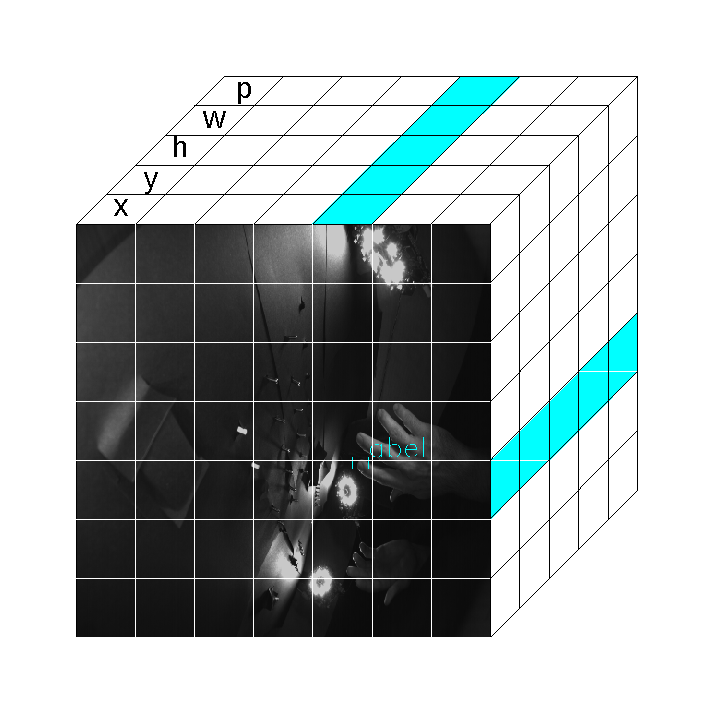
\includegraphics[width=.7\textwidth]{Kapitel/30DatenPipeline/Bilder/LabelTensor.pdf}
	\caption{Label-Tensor}
	\label{img:label_tensor}
\end{figure} 

\subsubsection{Liste von Label-Tensoren}
Diese Label-Tensoren enthalten alle wichtigen Labels von je einem Bild. 
Allerdings lassen Sie sich mit den darin enthaltenen Informationen nicht eindeutig einem Bild zuordnen. 
Um dies zu ermöglichen wurde eine Liste (Abbildung \ref{img:label_list}) erstellt, welche zwei Spalten und beliebig viele Zeilen enthält.
In der ersten Spalte wird der Name der zum Label gehörenden Bilddatei gespeichert, während in der zweiten Spalte der Label-Tensor selber gespeichert wird. 
Diese Liste wiederum wird mit pickle als python Objekt abgespeichert.
Der Speicherort dieser Liste ist derselbe wie derjenige, an welchem alle Bilder des entsprechenden Testsets oder Trainingsets abgespeichert wurden.

%Label-List
\begin{figure}	
	\centering
	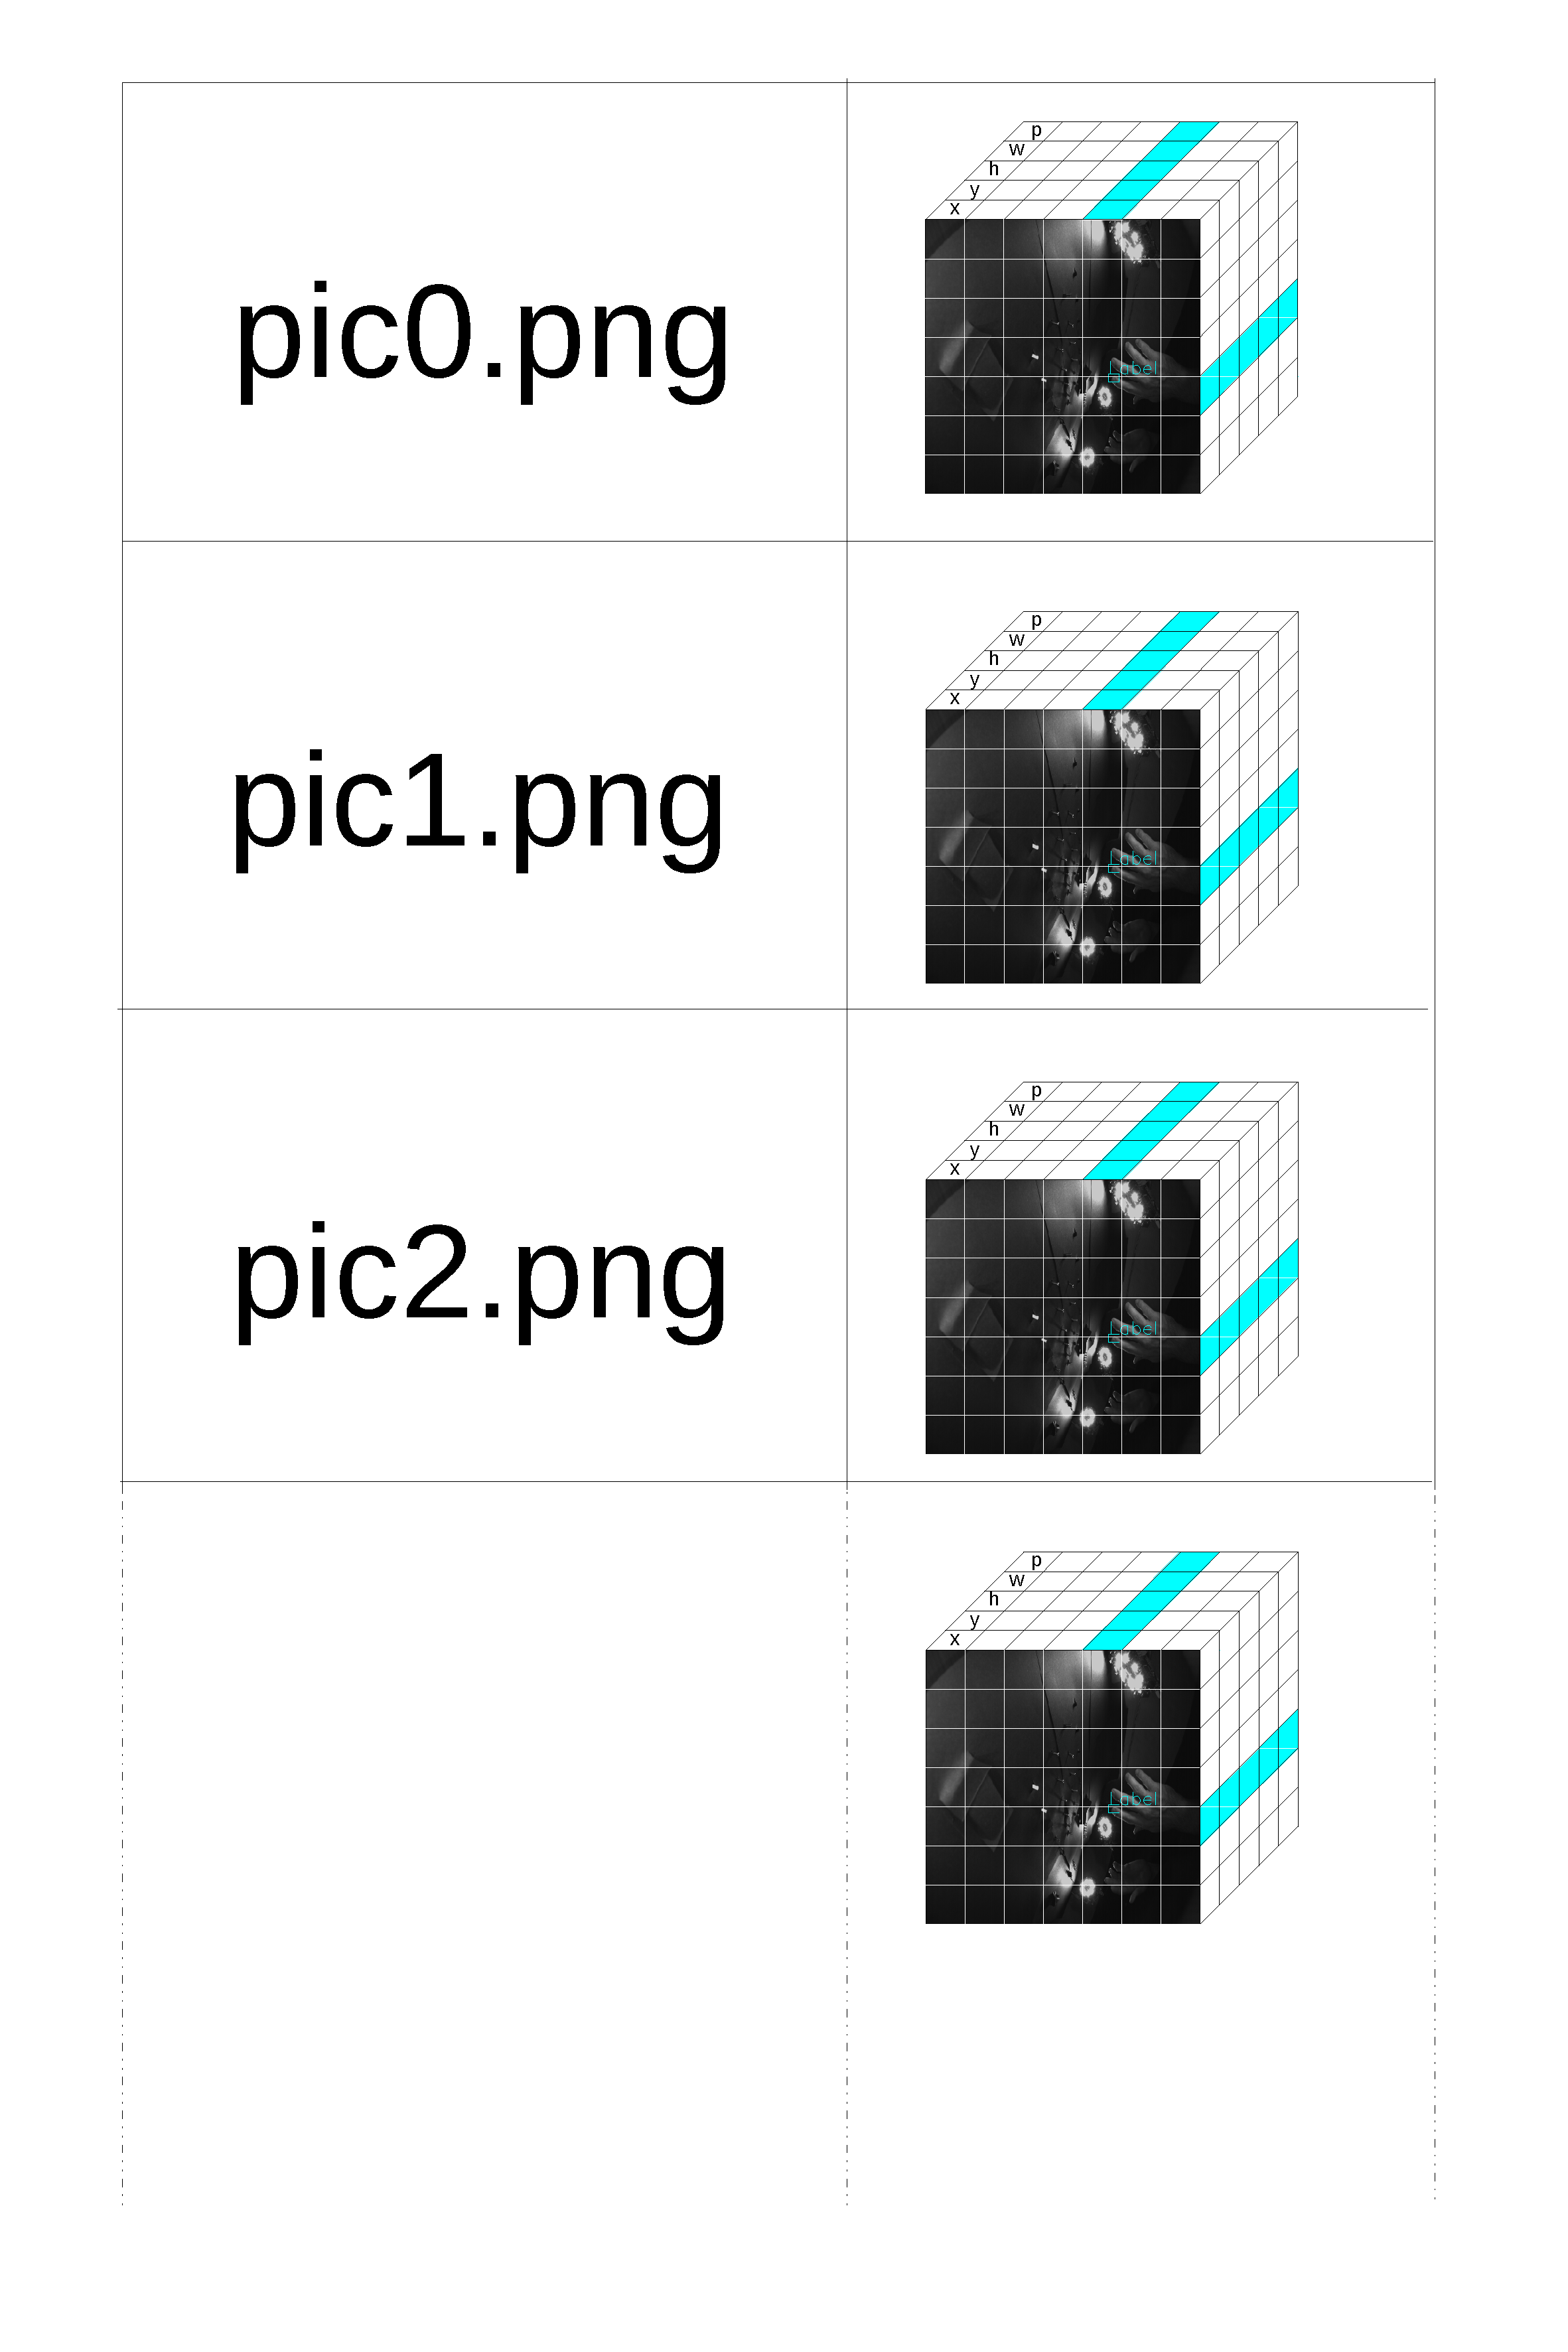
\includegraphics[width=.4\textwidth]{Kapitel/30DatenPipeline/Bilder/LabelList.pdf}
	\caption{Liste von Label-Tensoren}
	\label{img:label_list}
\end{figure} 
\subsection{Daten in Neuronales Netzwerk einlesen}
Das einlesen der Daten in das Programm, in welchem das Neuronale Netzwerk trainiert wird ist dank dem vorbereiteten Tensor und dessen Klasse, welche die Tensoren einfach laden lässt kein Problem. 
Die Daten schön für Tensorflow bereitzustellen ist etwas umständlich.
Dies aber nur bis man es mal zum laufen gebracht hat. 
Danach stellt dies kein Problem mehr dar. 
Bis die Bilder wirklich ins Netzwerk gefüttert werden passieren noch folgenden Punkte. 
\begin{enumerate}
\item Listen mit Bildnamen und Labels laden und als Tensorflow Datenset anlegen.
\item Einen \grqq{}Shuffler\grqq{} einfügen, der jedes Mal wenn das Neuronale Netzwerk einen neuen Minibatch verlangt die entsprechenden Daten Zufällig auswählt.
\item Eine Funktion, welche die Bildnamen durch die echten Bilder ersetzt. 
Der Vorteil einer solchen Funktion ist, dass die Bilder wirklich erst geladen werden, wenn die Daten auch benötigt werden. 
So werden im Punkt 2 nicht die schwergewichtigen Bilder sondern nur deren Namen aus der Liste durchgemischelt. 
\item Eine Funktion übernimmt das organisieren des Minibatches. 
So kann die Grösse des Minibatches flexibel bestimmt werden.
\item Die Bilder wurden von der Grösse 1280*960 auf 448*448 umgewandelt. 
Um diesen Punkt auf die GPU auszulagern wurde dafür eine eigenständige Tensorflow-Funktion verwendet (tf.image.resize\_images). 
\item Die Bilder wurden normalisiert. 
Dafür wurde eine eigene Funktion geschrieben, welche wiederum aus mehreren Tensorflow-Funktionen bestand. 
So wird auch dieser Task von der GPU erledigt.
\end{enumerate}
Die Punkte 1-3 waren mithilfe der Tensorflowklasse \grqq{}tf.contrib.data.Dataset\grqq{} relativ einfach zu bewältigen.
